\lesson{7}{Apr 16 2022 Sat (21:49:19)}{Part 4: Intro to Trig Functions}
\label{les_7:part_4_intro_to_trig_functions}

Recall that the sin and cos functions represent the coordinates of points in the
circumference of a unit circle. We found the values for $30^{\circ}$,
$45^{\circ}$, and $60^{\circ}$ by finding the coordinates of the points on the
circumference of the unit circle specified by these angles. The points we found
were all in Quadrant I, but since a circle is symmetric about both the $x$ and
$y$ axes, we can reflect these points about the coordinate axes to determine the
coordinates of corresponding points in the other quadrants. This means we can
use the sin and cos values of $\frac{\pi}{6}$, $\frac{\pi}{4}$, and
$\frac{\pi}{3}$ to find the sin and cos values of corresponding angles in other
quadrants.

Because of the symmetry of a circle, we can take a point in Quadrant I and
reflect it about the x-axis, the y-axis, and about both axes in order to obtain
corresponding points, one in each of the three other quadrants; the absolute
value of the coordinates of all four of these points is the same, i.e., they
only differ by their signs.

\begin{figure}[htpb]
  \centering

  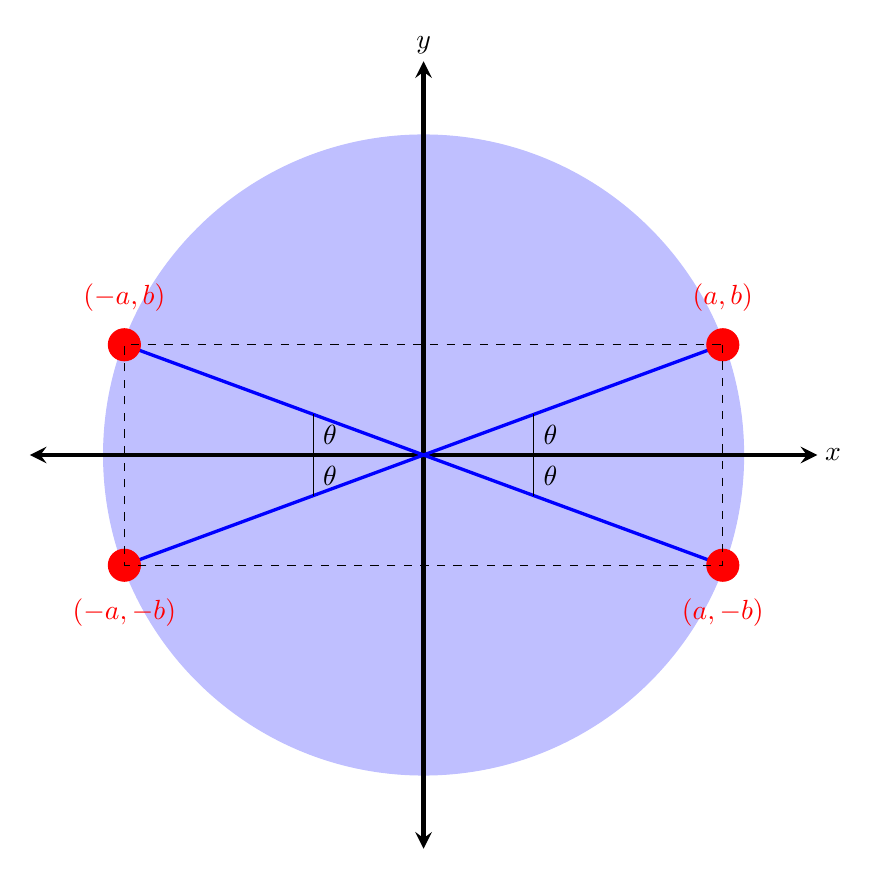
\begin{tikzpicture}
    % The main circle
    \draw[draw=blue!25!white,fill=blue!25!white] (0,0) circle (1.60in);

    % The x-y axis
    \draw (0,5.2) node[fill=white,anchor=center] {$y$};
    \draw (5.2,0) node[fill=white,anchor=center] {$x$};
    \draw[stealth-stealth,ultra thick] (0,5) -- (0,-5);
    \draw[stealth-stealth,ultra thick] (5,0) -- (-5,0);

    % The main angle line
    \draw[blue,very thick] (0,0) -- (3.8,1.4);
    \draw[blue,very thick] (0,0) -- (-3.8,1.4);
    \draw[blue,very thick] (0,0) -- (3.8,-1.4);
    \draw[blue,very thick] (0,0) -- (-3.8,-1.4);

    % Circling the point the line intersects the circumference
    \draw[draw=red,fill=red] (3.8,1.4) circle (0.08in);
    \draw[draw=red,fill=red] (-3.8,1.4) circle (0.08in);
    \draw[draw=red,fill=red] (3.8,-1.4) circle (0.08in);
    \draw[draw=red,fill=red] (-3.8,-1.4) circle (0.08in);

    % Rectangle covering the points
    \draw[dashed] (3.8,1.4) rectangle (-3.8,-1.4);

    \draw[red] (3.8,2) node[anchor=center] {$(a, b)$};
    \draw[red] (-3.8,2) node[anchor=center] {$(-a, b)$};
    \draw[red] (3.8,-2) node[anchor=center] {$(a, -b)$};
    \draw[red] (-3.8,-2) node[anchor=center] {$(-a, -b)$};

    % The angle of theta
    \draw (1.4,0.52) to node[right] {$\theta$} (1.4,0);
    \draw (-1.4,0.52) to node[right] {$\theta$} (-1.4,0);
    \draw (1.4,-0.52) to node[right] {$\theta$} (1.4,0);
    \draw (-1.4,-0.52) to node[right] {$\theta$} (-1.4,0);
  \end{tikzpicture}

  \caption{Plot of $(a, b)$ specified by angle $\theta$ with the other points in all the quadrants.}
  \label{fig:sin_cos_in_different_quadrants}
\end{figure}

Although all four of the points are specified by a different angle, all four of
the angles share the same reference angle, $\theta$.

\begin{definition}[Reference Angle]
  \label{def:reference_angle}

  The \textbf{reference angle} for an angle is the acute angle between the
  terminal side of the angle and the $x$-axis.
\end{definition}

\begin{exc}
  \label{exc:find_reference_angle_1}

  Find the reference angle for $150^{\circ}$ and $\frac{5\pi}{4}$.
\end{exc}

Now let's find out how we can use reference angles to determine the sin and cos
of any integer multiple of $\frac{\pi}{6}$, $\frac{\pi}{4}$ and
$\frac{\pi}{3}$.

\newpage
